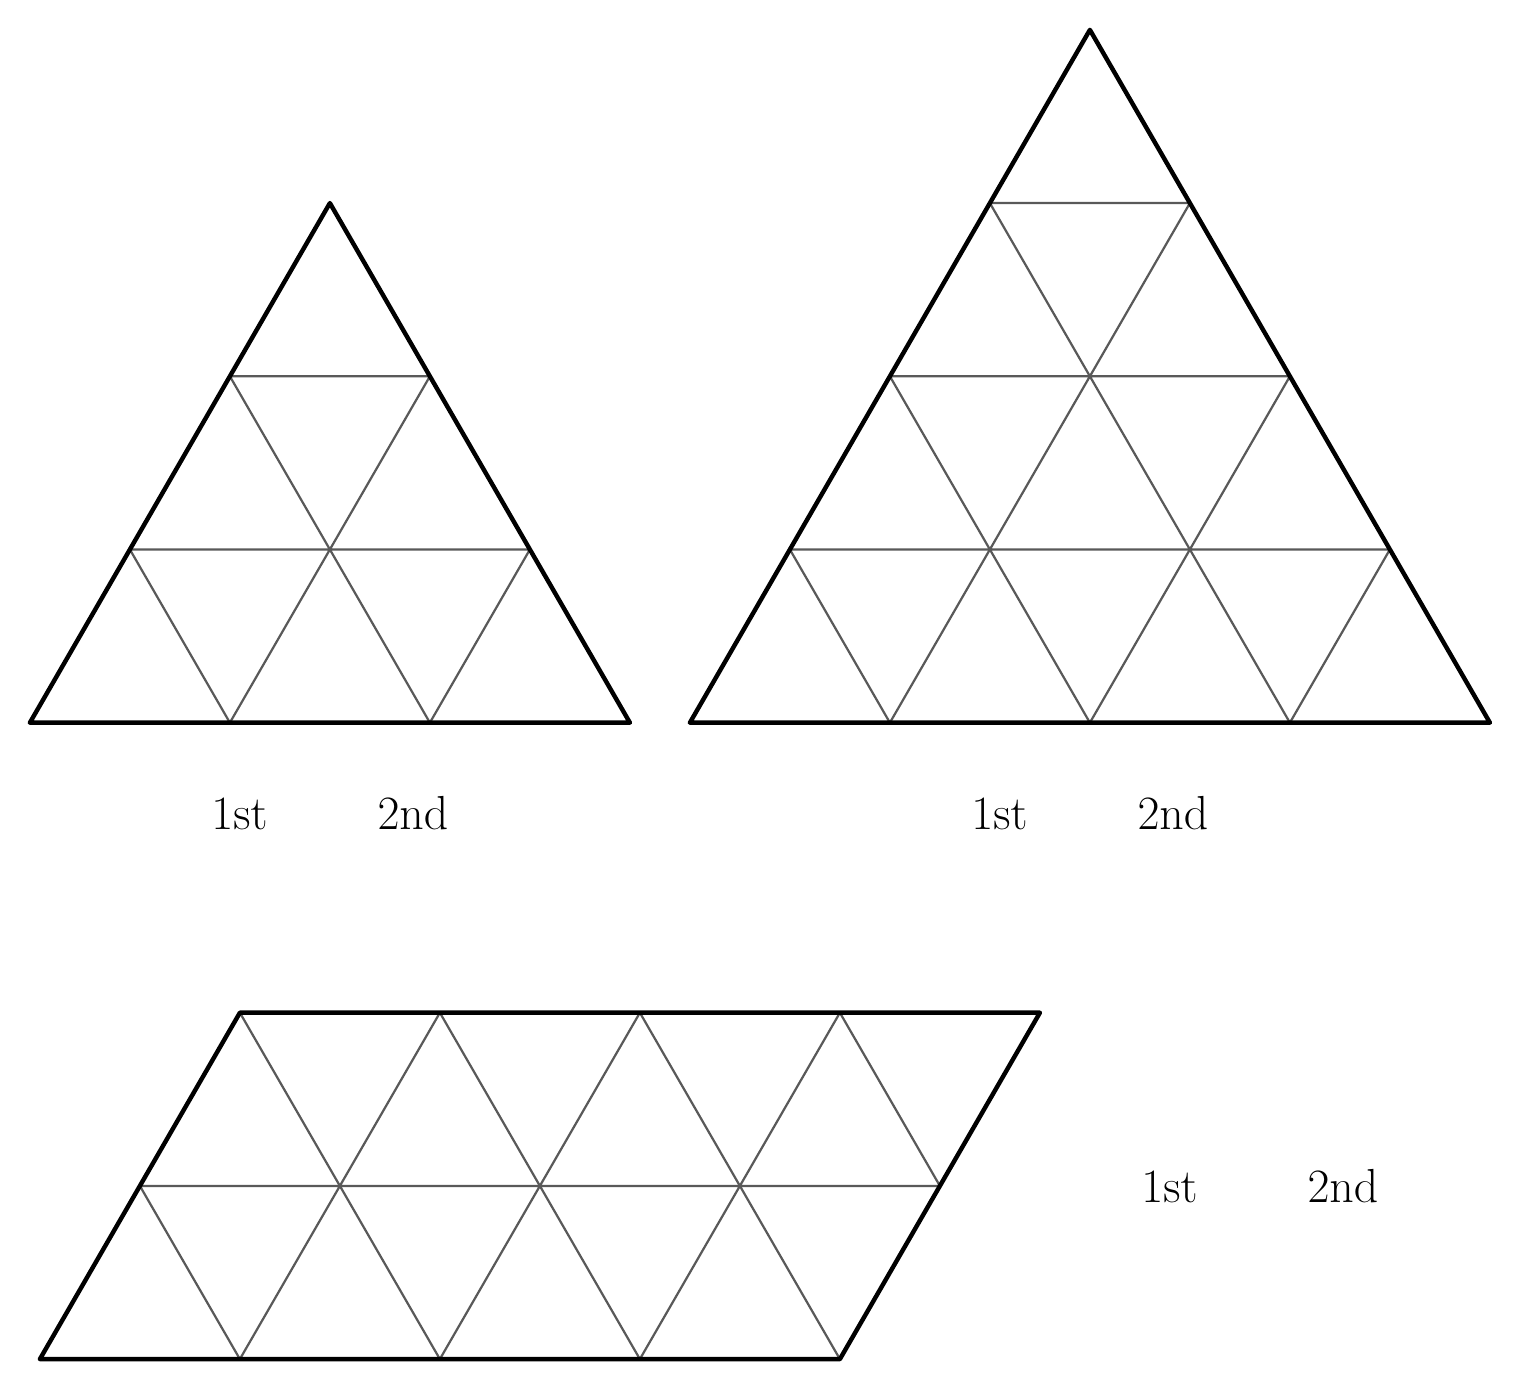
\begin{tikzpicture}[x=1in,y=1in]
\draw[line width=0.8pt, black!65] (1.2,0) -- (0.7,0.866) (0.7,0.866) -- (1.7,0.866) (1.2,0) -- (1.7,0.866) (1.7,0.866) -- (2.2,0) (1.7,0.866) -- (2.7,0.866) (2.2,0) -- (2.7,0.866) (2.7,0.866) -- (3.2,0) (3.7,0.866) -- (2.7,0.866) (3.7,0.866) -- (3.2,0) (3.7,0.866) -- (3.2,1.7321) (2.7,0.866) -- (3.2,1.7321) (3.7,0.866) -- (4.2,0) (3.7,0.866) -- (4.7,0.866) (1.7,0.866) -- (1.2,1.7321) (1.7,0.866) -- (2.2,1.7321) (2.2,1.7321) -- (2.7,0.866) (3.7,0.866) -- (4.2,1.7321) (4.2,1.7321) -- (4.7,0.866);
\draw[line width=1.6pt, black, line join=round] (4.2,0) -- (5.2,1.7321) -- (1.2,1.7321) -- (0.2,0) -- cycle;
\node[anchor=center, inner sep=0pt] at (6.3,0.866) {\LARGE 1st\hspace{0.55in}2nd};
\draw[line width=0.8pt, black!65] (1.65,4.0481) -- (2.15,3.1821) (1.15,3.1821) -- (1.65,4.0481) (1.15,3.1821) -- (0.65,4.0481) (0.65,4.0481) -- (1.65,4.0481) (1.15,4.9141) -- (2.15,4.9141) (1.65,4.0481) -- (2.65,4.0481) (2.15,3.1821) -- (2.65,4.0481) (1.65,4.0481) -- (1.15,4.9141) (1.65,4.0481) -- (2.15,4.9141);
\draw[line width=1.6pt, black, line join=round] (3.15,3.1821) -- (1.65,5.7801) -- (0.15,3.1821) -- cycle;
\node[anchor=center, inner sep=0pt] at (1.65,2.7321) {\LARGE 1st\hspace{0.55in}2nd};
\draw[line width=0.8pt, black!65] (4.45,3.1821) -- (3.95,4.0481) (3.95,4.0481) -- (4.95,4.0481) (4.45,3.1821) -- (4.95,4.0481) (4.45,4.9141) -- (5.45,4.9141) (5.45,4.9141) -- (4.95,5.7801) (4.95,4.0481) -- (5.45,3.1821) (4.95,4.0481) -- (5.95,4.0481) (5.45,3.1821) -- (5.95,4.0481) (5.45,4.9141) -- (6.45,4.9141) (5.45,4.9141) -- (5.95,5.7801) (5.95,4.0481) -- (6.45,3.1821) (6.95,4.0481) -- (5.95,4.0481) (6.95,4.0481) -- (6.45,3.1821) (5.95,4.0481) -- (6.45,4.9141) (4.95,4.0481) -- (4.45,4.9141) (4.95,4.0481) -- (5.45,4.9141) (5.45,4.9141) -- (5.95,4.0481) (4.95,5.7801) -- (5.95,5.7801);
\draw[line width=1.6pt, black, line join=round] (3.45,3.1821) -- (7.45,3.1821) -- (5.45,6.6462) -- cycle;
\node[anchor=center, inner sep=0pt] at (5.45,2.7321) {\LARGE 1st\hspace{0.55in}2nd};
\end{tikzpicture}
